% Options for packages loaded elsewhere
\PassOptionsToPackage{unicode}{hyperref}
\PassOptionsToPackage{hyphens}{url}
%
\documentclass[
  english,
  symmetric,justified,marginals=raggedouter]{tufte-book}
\usepackage[]{mathpazo}
\usepackage{amssymb,amsmath}
\usepackage{ifxetex,ifluatex}
\ifnum 0\ifxetex 1\fi\ifluatex 1\fi=0 % if pdftex
  \usepackage[T1]{fontenc}
  \usepackage[utf8]{inputenc}
  \usepackage{textcomp} % provide euro and other symbols
\else % if luatex or xetex
  \usepackage{unicode-math}
  \defaultfontfeatures{Scale=MatchLowercase}
  \defaultfontfeatures[\rmfamily]{Ligatures=TeX,Scale=1}
\fi
% Use upquote if available, for straight quotes in verbatim environments
\IfFileExists{upquote.sty}{\usepackage{upquote}}{}
\IfFileExists{microtype.sty}{% use microtype if available
  \usepackage[]{microtype}
  \UseMicrotypeSet[protrusion]{basicmath} % disable protrusion for tt fonts
}{}
\usepackage{xcolor}
\IfFileExists{xurl.sty}{\usepackage{xurl}}{} % add URL line breaks if available
\IfFileExists{bookmark.sty}{\usepackage{bookmark}}{\usepackage{hyperref}}
\hypersetup{
  pdfauthor={Wouter Groeneveld},
  pdflang={en},
  hidelinks,
  pdfcreator={LaTeX via pandoc}}
\urlstyle{same} % disable monospaced font for URLs
\providecommand{\tightlist}{%
  \setlength{\itemsep}{0pt}\setlength{\parskip}{0pt}}
\setcounter{secnumdepth}{-\maxdimen} % remove section numbering
\hypersetup{colorlinks}
\usepackage{etoolbox}

%% 
% xelatex tufte fixes 
% https://tex.stackexchange.com/questions/202142/problems-compiling-tufte-title-page-in-xelatex
\renewcommand{\textls}[2][5]{%
  \begingroup\addfontfeatures{LetterSpace=#1}#2\endgroup
}
\renewcommand{\allcapsspacing}[1]{\textls[15]{#1}}
\renewcommand{\smallcapsspacing}[1]{\textls[10]{#1}}
\renewcommand{\allcaps}[1]{\textls[15]{\MakeTextUppercase{#1}}}
\renewcommand{\smallcaps}[1]{\smallcapsspacing{\scshape\MakeTextLowercase{#1}}}
\renewcommand{\textsc}[1]{\smallcapsspacing{\textsmallcaps{#1}}}


%%
% usepackage won't work, already included in docclass?
% paperwidth =  left + width + right                        185
%   width = textwidth (+ marginparsep + marginparwidth)     158
% paperheight = top + height + bottom                       225
%   height = textheight (+ headheight + headsep + footskip) 205
\geometry{
  %showframe,
  twoside,
  includemp,
  includehead,
  includefoot,
  %,
  paperwidth=185mm,
  textwidth=104mm,
  marginparsep=4mm,
  marginparwidth=50mm,
  inner=12mm,
  outer=15mm,
  %,
  paperheight=225mm,
  textheight=195mm,
  headheight=10mm,
  headsep=10mm,
  footskip=0mm,
  top=5mm,
  bottom=15mm
}
%%
% Book metadata
\title{A Tufte-Style Book\thanks{Thanks to Edward R.~Tufte for his inspiration.}}
\author[The Tufte-LaTeX Developers]{The Tufte-LaTeX\ Developers}
\publisher{Publisher of This Book}

%%
% Prints a trailing space in a smart way.
\usepackage{xspace}

% ===================
% = Font/Text Setup =
% ===================
% The fancyvrb package lets us customize the formatting of verbatim
% environments.  We use a slightly smaller font.
\usepackage{fancyvrb}
\fvset{fontsize=\normalsize}

%%
% xelatex-specific font setup - main: mathpazo-style
\usepackage{fontspec}
\setmainfont
     [ BoldFont       = texgyrepagella-bold.otf ,
       ItalicFont     = texgyrepagella-italic.otf ,
       BoldItalicFont = texgyrepagella-bolditalic.otf ]
     {texgyrepagella-regular.otf}
\newfontfamily{\retro}{SuperLegendBoy}[Extension = .ttf]
% for Japanese chars - not needed (yet)
% \usepackage{xeCJK}
% \setCJKmainfont[BoldFont=STHeiti,ItalicFont=STKaiti]{STSong}

% set chapter/section/quote styles to retro font
\usepackage{sectsty}
\chapterfont{\retro}
\sectionfont{\retro}
\subsectionfont{\retro}
\AtBeginEnvironment{quote}{\retro}

\renewcommand{\labelitemi}{$\circ$}

% ================
% = Images Setup =
% ================
% for png/pdf inclusion (pdfpages: full-page)
\usepackage{graphicx}
\graphicspath{{img/}}
\setkeys{Gin}{width=\linewidth,totalheight=\textheight,keepaspectratio}

% figure caption styles. tufte-book is incompatible with package caption...
% https://tex.stackexchange.com/questions/106416/remove-prefix-from-figure-caption-in-tufte-book-document-class
\makeatletter
\patchcmd{\@caption}
  {\noindent\csname fnum@#1\endcsname: \ignorespaces}
  {}
  {}{}
\makeatother

\newcommand\cover[4]{
  \begin{marginfigure}[5cm] % assumes \cover is called right after a new chapter.
    \includegraphics[width=\linewidth]{covers/#1.jpg}
    \caption{\textbf{Developer}: #2 \newline \textbf{Release}: #3 \newline \textbf{Genre}: #4}
    \label{fig:marginfig}
  \end{marginfigure}  
}


%% 
% background test (use \BgThispage on page if 'some' option enabled)
%\usepackage[pages=some]{background}
%\backgroundsetup{
%  scale=1.1,
%  angle=0,
%  opacity=1,  %% adjust
%  contents={\includegraphics[width=\paperwidth,height=\paperheight]{chapters/wario4.png}}
%}

%% 
% begin new chapter left-side (complications with tufte-book)
%\makeatletter
%\renewcommand*\cleardoublepage{\clearpage\if@twoside
%  \ifodd\c@page \hbox{}\newpage\if@twocolumn\hbox{}%
%  \newpage\fi\fi\fi}
%\makeatother

% Generates the index
\usepackage{makeidx}
\makeindex

%%
% Tufte shortcuts, copied from sample-book.tex
% Prints the month name (e.g., January) and the year (e.g., 2008)
\newcommand{\monthyear}{%
  \ifcase\month\or January\or February\or March\or April\or May\or June\or
  July\or August\or September\or October\or November\or
  December\fi\space\number\year
}

\newenvironment{docspec}{\begin{quotation}\ttfamily\parskip0pt\parindent0pt\ignorespaces}{\end{quotation}}% command specification environment


% Prints an epigraph and speaker in sans serif, all-caps type.
\newcommand{\openepigraph}[2]{%
  %\sffamily\fontsize{14}{16}\selectfont
  \begin{fullwidth}
  \sffamily\large
  \begin{doublespace}
  \noindent\allcaps{#1}\\% epigraph
  \noindent\allcaps{#2}% author
  \end{doublespace}
  \end{fullwidth}
}

\ifxetex
  % Load polyglossia as late as possible: uses bidi with RTL langages (e.g. Hebrew, Arabic)
  \usepackage{polyglossia}
  \setmainlanguage[]{english}
\else
  \usepackage[shorthands=off,main=english]{babel}
\fi
\usepackage[]{natbib}
\bibliographystyle{plainnat}

\author{Wouter Groeneveld}
\date{2019-06-12}

\begin{document}
\frontmatter


% r.3 full title page
\maketitle


% v.4 copyright page
\newpage
\begin{fullwidth}
~\vfill
\thispagestyle{empty}
\setlength{\parindent}{0pt}
\setlength{\parskip}{\baselineskip}
Copyright \copyright\ \the\year\ \thanklessauthor

\par\smallcaps{Published by \thanklesspublisher}

\par\smallcaps{tufte-latex.googlecode.com}

\par Licensed under the Apache License, Version 2.0 (the ``License''); you may not
use this file except in compliance with the License. You may obtain a copy
of the License at \url{http://www.apache.org/licenses/LICENSE-2.0}. Unless
required by applicable law or agreed to in writing, software distributed
under the License is distributed on an \smallcaps{``AS IS'' BASIS, WITHOUT
WARRANTIES OR CONDITIONS OF ANY KIND}, either express or implied. See the
License for the specific language governing permissions and limitations
under the License.\index{license}

\par\textit{First printing, \monthyear}
\end{fullwidth}

% r.5 contents
\tableofcontents


% r.7 dedication
\cleardoublepage
~\vfill
\begin{doublespace}
\noindent\fontsize{18}{22}\selectfont\itshape
\nohyphenation
Dedicated to those who appreciate \LaTeX{} 
and the work of \mbox{Edward R.~Tufte} 
and \mbox{Donald E.~Knuth}.
\end{doublespace}
\vfill
\vfill

% r.9 introduction
\cleardoublepage


\mainmatter
\frontmatter

\hypertarget{voorwoord}{%
\chapter{Voorwoord}\label{voorwoord}}

\newthought{In tijden waarin} elk nieuwste hebbeding, bekend persoon of online
fenomeen quasi meteen wordt uitgeroepen tot de tweede komst van Christus
- laten we eerlijk wezen, ondertussen niet meer dan een ordinaire
marketingtruc- durf ik te stellen dat Wouter Groeneveld een van de
weinigen is die aanspraak mag maken op deze blijkbaar felbegeerde titel.
Wouter bekwaamde zich de afgelopen jaren dan ook uitermate in Jezus'
meest opvallende handelsmerk: het vermenigvuldigen en vervolgens delen
van brood. Ik maak de uiteindelijke keuze niet maar volgens mij verdient
dat een van de meer luxueuzere plekken in wat er ook na dit leven komt.

Blabla new alinea citatie \cite{dreyfus1980five}.

\mainmatter

\hypertarget{x}{%
\chapter{X}\label{x}}

\cover{x}{Argonaut Games}{1992 (JPN)}{Space combat simulator}

\newthought{X is a} 1992 space combat simulator video game developed by Argonaut
Games and published by Nintendo for the Game Boy in Japan. The player
assumes the role of the VIXIV starship as it must protect the planet
Tetamus II from a mysterious race of aliens. Gameplay involves
completing missions assigned by the ``Training Academy Coach'', ranging
from protecting bases from enemy fire or delivering cargo to a certain
area.

\begin{quote}
En toen was dat kapot boem zei het - dylan
\end{quote}

Notable for being one of the few attempts at a 3D video game on the Game
Boy alongside Faceball 2000, X was the creation of Dylan Cuthbert, who
would later design the original Star Fox for the Super NES. Commissioned
by Argonaut president Jez San after being impressed by the Game Boy at
the 1991 Consumer Electronics Show, Cuthbert and a team of others were
forced to reverse-engineer the system due to official development kits
being hard to find. It was designed after Argonaut's earlier game
Starglider 2 for the Amiga. Nintendo grew interested in the game during
production and convinced Cuthbert and Argonaut to make it a first-party
title for the console. A planned North American release named Lunar
Chase was cancelled as Nintendo of America felt a game of its type was
too advanced for a console meant for children.

X initially received mixed reviews from critics, often being praised for
its impressive technological accomplishments but criticized for its high
difficulty. Retrospectively, it was acclaimed for its historical
importance and gameplay, often being compared to games such as Star
Luster. A DSiWare sequel, X-Scape, was released worldwide in 2010.

\hypertarget{de-boer-de-molenaar-en-de-brouwer}{%
\chapter{De boer, de molenaar en de
brouwer}\label{de-boer-de-molenaar-en-de-brouwer}}

\newthought{The pages of} a book are usually divided into three major sections: the
front matter (also called preliminary matter or prelim), the main matter
(the core text of the book), and the back matter (or end matter).

\begin{marginfigure}%
  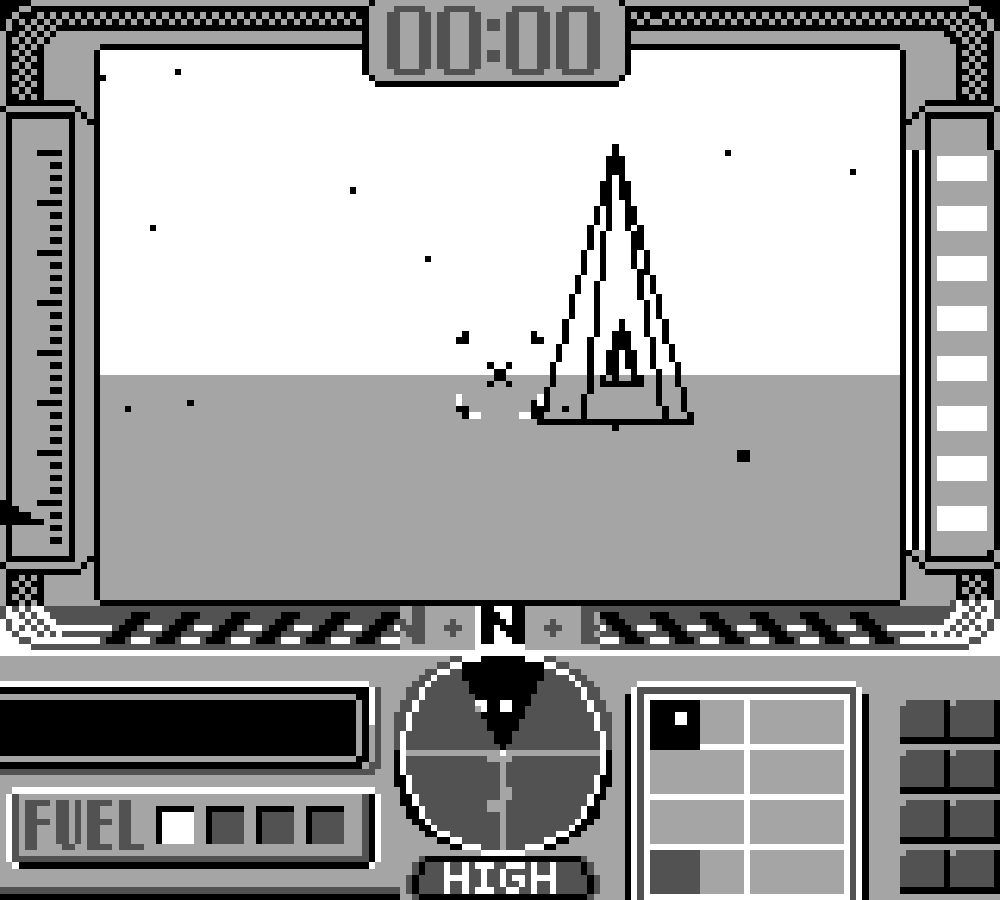
\includegraphics[width=\linewidth]{x.png}
  \caption{Spelleke X in margin.}
  \label{fig:marginfig}
\end{marginfigure}

\hypertarget{nieuwe-gedachtes}{%
\section{Nieuwe gedachtes}\label{nieuwe-gedachtes}}

The pages of a book are usually divided into three major sections: the
front matter (also called preliminary matter or prelim), the main matter
(the core text of the book), and the back matter (or end matter).

Tufte's books include the following heading levels: parts,
chapters,\sidenote{Parts and chapters are defined for the \texttt{tufte-book}
class only.} sections, subsections, and paragraphs. Not defined by
default are: sub-subsections and subparagraphs.

\hypertarget{een}{%
\subsection{Een}\label{een}}

Quis magna Lorem anim amet ipsum do mollit sit cillum voluptate ex nulla
tempor. Laborum consequat non elit enim exercitation cillum aliqua
consequat id aliqua. Esse ex consectetur mollit voluptate est in duis
laboris ad sit ipsum anim Lorem. Incididunt veniam velit elit elit
veniam Lorem aliqua quis ullamco deserunt sit enim elit aliqua esse
irure. Laborum nisi sit est tempor laborum mollit labore officia laborum
excepteur commodo non commodo dolor excepteur commodo. Ipsum fugiat ex
est consectetur ipsum commodo tempor sunt in proident.

Tufte's books include the following heading levels: parts,
chapters,\sidenote{Parts and chapters are defined for the \texttt{tufte-book}
class only.} sections, subsections, and paragraphs. Not defined by
default are: sub-subsections and subparagraphs.

\hypertarget{twee}{%
\subsection{Twee}\label{twee}}

Quis magna Lorem anim amet ipsum do mollit sit cillum voluptate ex nulla
tempor. Laborum consequat non elit enim exercitation cillum aliqua
consequat id aliqua. Esse ex consectetur mollit voluptate est in duis
laboris ad sit ipsum anim Lorem. Incididunt veniam velit elit elit
veniam Lorem aliqua quis ullamco deserunt sit enim elit aliqua esse
irure. Laborum nisi sit est tempor laborum mollit labore officia laborum
excepteur commodo non commodo dolor excepteur commodo. Ipsum fugiat ex
est consectetur ipsum commodo tempor sunt in proident.

\begin{figure*}[h]
  \includegraphics[width=\linewidth]{wario4.png}%
  \caption{This graph shows $y = \sin x$ from about $x = [-10, 10]$.
  \emph{Notice that this figure takes up the full page width.}}%
  \label{fig:fullfig}%
\end{figure*}

\begin{docspec}
\textbackslash begin\{marginfigure\}\\
  \qquad\textbackslash includegraphics\{helix\}\\
  \qquad\textbackslash caption\{This is a margin figure.\}\\
  \qquad\textbackslash label\{fig:marginfig\}\\
\textbackslash end\{marginfigure\}\\
\end{docspec}

\begin{marginfigure}%
  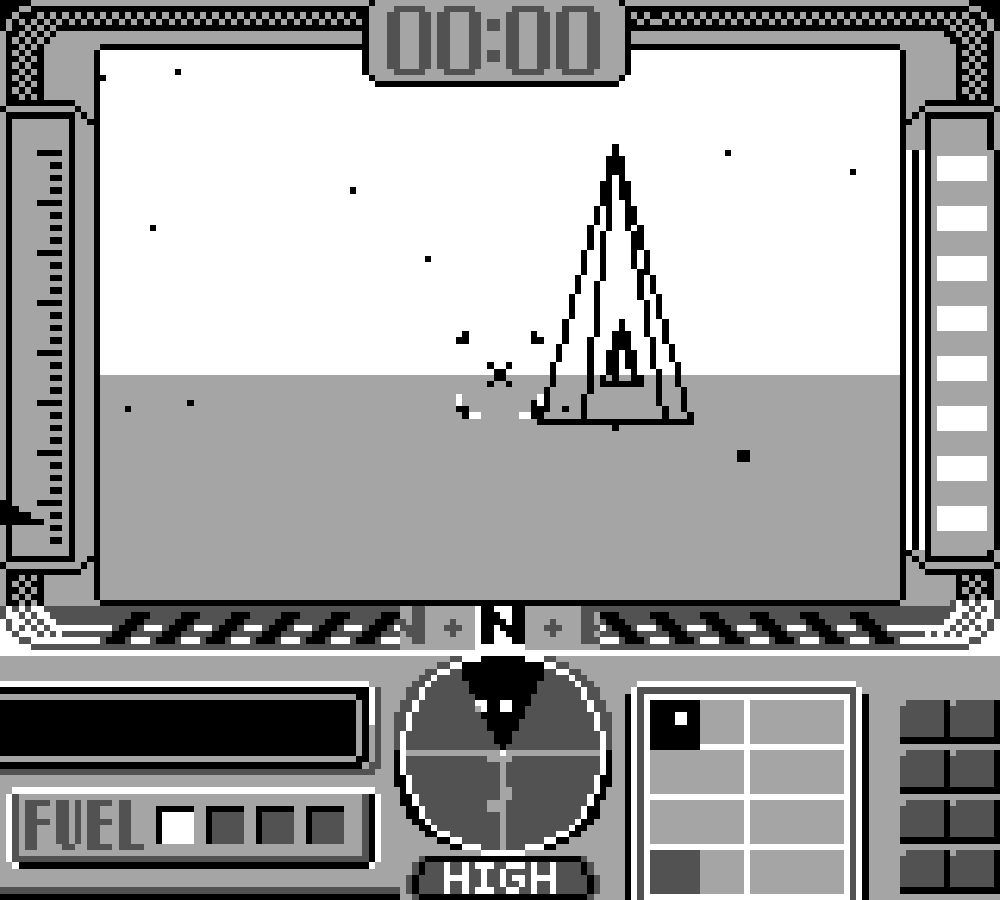
\includegraphics[width=\linewidth]{x.png}
  \caption{Spelleke X in margin.}
  \label{fig:marginfig}
\end{marginfigure}

Quis magna Lorem anim amet ipsum do mollit sit cillum voluptate ex nulla
tempor. Laborum consequat non elit enim exercitation cillum aliqua
consequat id aliqua. Esse ex consectetur mollit voluptate est in duis
laboris ad sit ipsum anim Lorem. Incididunt veniam velit elit elit
veniam Lorem aliqua quis ullamco deserunt sit enim elit aliqua esse
irure. Laborum nisi sit est tempor laborum mollit labore officia laborum
excepteur commodo non commodo dolor excepteur commodo. Ipsum fugiat ex
est consectetur ipsum commodo tempor sunt in proident.

\newthought{In his later books}, Quis magna Lorem anim amet ipsum do
mollit sit cillum voluptate ex nulla tempor. Laborum consequat non elit
enim exercitation cillum aliqua consequat id aliqua. Esse ex consectetur
mollit voluptate est in duis laboris ad sit ipsum anim Lorem. Incididunt
veniam velit elit elit veniam Lorem aliqua quis ullamco deserunt sit
enim elit aliqua esse irure. Laborum nisi sit est tempor laborum mollit
labore officia laborum excepteur commodo non commodo dolor excepteur
commodo. Ipsum fugiat ex est consectetur ipsum commodo tempor sunt in
proident.

\begin{figure}[h!]
  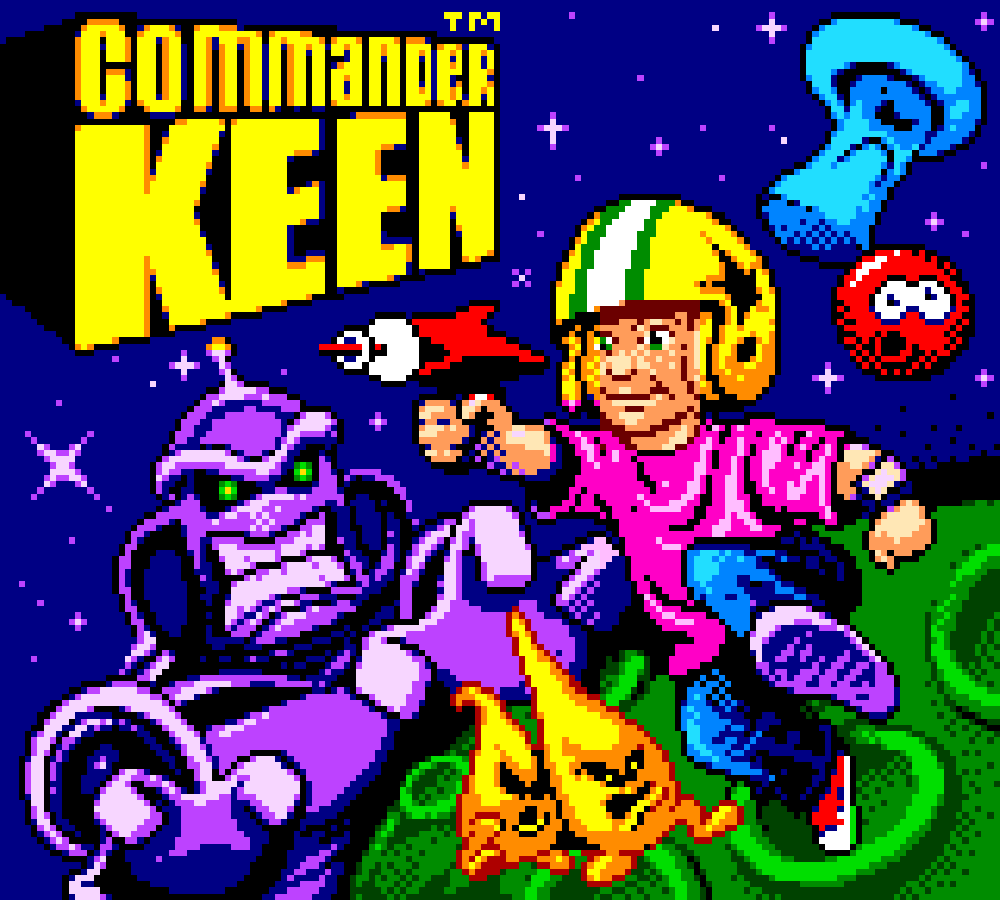
\includegraphics{keen.png}
%  \checkparity This is an \pageparity\ page.%
  \caption[Hilbert curves of various degrees $n$.][6pt]{Hilbert curves of various degrees $n$. \emph{Notice that this figure only takes up the main textblock width.}}
  \label{fig:textfig}
  %\zsavepos{pos:textfig}
\end{figure}

\begin{fullwidth}
Lorem ipsum dolor sit amet, consectetuer adipiscing elit. Ut purus elit, vestibulum ut, placerat ac, adipiscing vitae, felis. Curabitur
dictum gravida mauris. Nam arcu libero, nonummy eget, consectetuer id, vulputate a, magna. Donec vehicula augue eu neque.
Pellentesque habitant morbi tristique senectus et netus et malesuada fames ac turpis egestas. Mauris ut leo. Cras viverra metus
rhoncus sem. Nulla et lectus vestibulum urna fringilla ultrices. Phasellus eu tellus sit amet tortor gravida placerat. Integer sapien
est, iaculis in, pretium quis, viverra ac, nunc. Praesent eget sem vel leo ultrices bibendum. Aenean faucibus. Morbi dolor nulla,
malesuada eu, pulvinar at, mollis ac, nulla. Curabitur auctor semper nulla. Donec varius orci eget risus. Duis nibh mi, congue eu,
accumsan eleifend, sagittis quis, diam. Duis eget orci sit amet orci dignissim rutrum.
\end{fullwidth}

\backmatter

\small

  \bibliography{boek.bib}


\normalsize


\cleardoublepage

%\bibliography

% \addcontentsline{toc}{chapter}{\listfigurename} - already added to toc?
% https://texblog.org/2011/09/09/10-ways-to-customize-tocloflot/
\addtocontents{lof}{%
Beeldmateriaal gepubliceerd met toestemming. Figuren zonder expliciete vermelding van het \textcopyright \: teken zijn gemaakt door de auteur, waarvan alle rechten tevens zijn voorbehouden.
}
\listoffigures 
\listoftables
\end{document}